%%%%%%%%%%%%%%%%%%%%%%%%%%%%%%%%%%%%%%%%%%%%%%%%%%%%%%%%%%%%
\chapternonum{Introduction}
\nopagebreak
%%%%%%%%%%%%%%%%%%%%%%%%%%%%%%%%%%%%%%%%%%%%%%%%%%%%%%%%%%%%

%%%%%%%% Quote
%\begin{flushright}
%\parbox[h]{4.in}{{\small{\em 
%%The greatest challenge today, not just in cell biology and ecology but in all
%%of science, is the accurate and complete description of complex
%%systems. Scientist have broken down many kinds of systems. They think they
%%know most of the elements and forces. The next task is to reassemble them, at
%%least in mathematical models that capture the key properties of the entire ensembles
%
%Professor Hubert Farnsworth: Good Lord! That's over 5000 atmospheres of pressure!\\
%Fry: How many atmospheres can the ship withstand?\\
%Professor Hubert Farnsworth: Well, it was built for space travel, so anywhere between zero and one.\\
%\ \\ 
%Ludwig Boltzmann, who spent much of his life studying statistical mechanics,
%dies in 1906, by his own hand.\\
%Paul Ehrenfest, carrying on the work, died similarly in 1933.\\
%Now it's our turn to study statistical mechanics. Perhaps it will be wise to approach
%the subject cautiously.\\
%David Goodstein - \emph{State of Matter}, 1975, Dover N.Y.
%}}
%%\begin{flushright}
%%{\small Edward O. Wilson \cite{Wilson}.}
%%\end{flushright}
%}
%\end{flushright}


\paragraph{} %senza questo non funziona il correttore ortografico nel resto
\lettrine{T}{his} Thesis 
% focus on the application of the tools of
% Statistical Mechanics to the study and analysis of two different and relevant problems in modern molecular biology: 
% %biological systems. In particular we will focus in  
% the problem of protein sequencing by mass spectrometry and the  problem of 
% protein folding, with a special focus on the study of a modular protein.
% %in particular  of in the case of modular polymers.
addresses
%attempt to characterize 
two different %apparently unlike 
biological
problems with a common statistical-mechanics approach: in the first case we focus
on the problem of peptide
sequencing by {\sl de-novo} interpretation of Tandem %in the field of 
Mass spectra, while in the second we 
analyse the folding behaviour of Myotrophin, a small repeat protein that has been recently characterized by different experimental techniques.

Both problems, as the majority of  biologically relevant systems and processes,
are too complex to be approached in a detailed, \emph{ab-initio} way, based on a
reliable, microscopic description of the interactions and fundamental processes
involved; on the contrary, typically 
% Actually the majority of the biological interesting processes are too complex
% for a deep study based in its fundamental constituents and the driving forces acting
% on them, in exchange 
one has to resort to  %rely on 
various simplifications in the modelling of the original system, introducing, as
a consequence,  some approximations in order to achieve treatability. 
Hence,  the typical approach to the description of a biological system from a statistical-mechanics %physical
point of view starts with the research of a successful mapping of the
original complex problem to a treatable physical model, possibly involving coarse-graining or other kind of simplifications. 
%usually based on statistical mechanics, at different levels of details retain. 


In our case, the mapping of the above mentioned problems to 
%The map of each of those cases to a 
suitable statistical mechanical systems is performed
through the definition of the interesting dynamic variables and of an
energy function which determines their behaviour.
Moreover, for both problems we enforce a modelling of the interactions that 
% The resulting system, if breakable in subsystems that present interaction only
% with first neighbours, 
is amenable of an exact solution for the equilibrium
probability distribution through the Transfer Matrix Method.

Both problems are related to proteins: their identification with MS/MS and their folding. In the following, we resume some basic facts about such important biomolecules: their synthesis, their structure and their role in cellular processes.
% In the following we rely on this characteristic to take an insight in the system
% behaviour and its different conformations.

\paragraph{What is a Protein?}
Proteins are ubiquitous molecules in living cells, involved in almost all the
biochemical processes that govern their evolution.
Proteins are linear polymeric  chains,
composed by different combinations of 20 types of amino acids, covalently linked  in a sequence (the ``primary structure'') that completely encodes their three-dimensional structure and function. 
Each protein is completely characterized by its sequence, whose length may vary
between a few tens to several hundred ``residues'', as the amino acids are
called within the protein chain (the name acknowledges the fact that  they loose
a water molecule upon binding in the main chain).
% 
% This long chain of residues folds usually to a given, usually globular,
% three-dimensional structure, acquiring a functional role.

Protein synthesis is performed inside the cell through a DNA translation
mechanism,  based on the information contained in  the regions of the chromosomes corresponding to the genes.
The information on protein composition is, in fact, encoded into the DNA double
helix. The latter is found packed in the cell nucleus and is locally unpacked
``on demand'' and copied to a messenger mRNA strand (DNA transcription).
The mRNA strand exits the nucleus to reach the cytoplasm where the ribosomes are
located;  here, it can
undergo some modification (removal of the introns, alternative splicing) before being translated to a polypeptide chain.
Ribosomes decode the messenger RNA using the tri-nucleotide translation rules, that assign to each triplet
of RNA basis (``codons'') a specific residue to be appended to the peptide chain.

Once the amino acid chain is built up, it undergoes the process of folding to reach
its functional three-dimensional structure (the ``native structure''), which  is usually a precisely determined compact structure.
Often at this stage  the  newly formed protein undergoes some modification, mainly
characterized by the addiction of functional groups to polypeptide chain.
Notice that these changes cannot be read from the genetic code of the DNA, and depend on the specific cell conditions at the moment the protein is synthesized. 


\begin{figure}
\centering
\def\svgwidth{0.8\textwidth}
%% Creator: Inkscape inkscape 0.48.2, www.inkscape.org
%% PDF/EPS/PS + LaTeX output extension by Johan Engelen, 2010
%% Accompanies image file 'dna-transcription-translation-divided-text.eps' (pdf, eps, ps)
%%
%% To include the image in your LaTeX document, write
%%   \input{<filename>.pdf_tex}
%%  instead of
%%   \includegraphics{<filename>.pdf}
%% To scale the image, write
%%   \def\svgwidth{<desired width>}
%%   \input{<filename>.pdf_tex}
%%  instead of
%%   \includegraphics[width=<desired width>]{<filename>.pdf}
%%
%% Images with a different path to the parent latex file can
%% be accessed with the `import' package (which may need to be
%% installed) using
%%   \usepackage{import}
%% in the preamble, and then including the image with
%%   \import{<path to file>}{<filename>.pdf_tex}
%% Alternatively, one can specify
%%   \graphicspath{{<path to file>/}}
%% 
%% For more information, please see info/svg-inkscape on CTAN:
%%   http://tug.ctan.org/tex-archive/info/svg-inkscape
%%
\begingroup%
  \makeatletter%
  \providecommand\color[2][]{%
    \errmessage{(Inkscape) Color is used for the text in Inkscape, but the package 'color.sty' is not loaded}%
    \renewcommand\color[2][]{}%
  }%
  \providecommand\transparent[1]{%
    \errmessage{(Inkscape) Transparency is used (non-zero) for the text in Inkscape, but the package 'transparent.sty' is not loaded}%
    \renewcommand\transparent[1]{}%
  }%
  \providecommand\rotatebox[2]{#2}%
  \ifx\svgwidth\undefined%
    \setlength{\unitlength}{522.10136108bp}%
    \ifx\svgscale\undefined%
      \relax%
    \else%
      \setlength{\unitlength}{\unitlength * \real{\svgscale}}%
    \fi%
  \else%
    \setlength{\unitlength}{\svgwidth}%
  \fi%
  \global\let\svgwidth\undefined%
  \global\let\svgscale\undefined%
  \makeatother%
%  \begin{picture}(1,0.36337107)%
  \begin{picture}(1,0.37)%
    \put(0,0){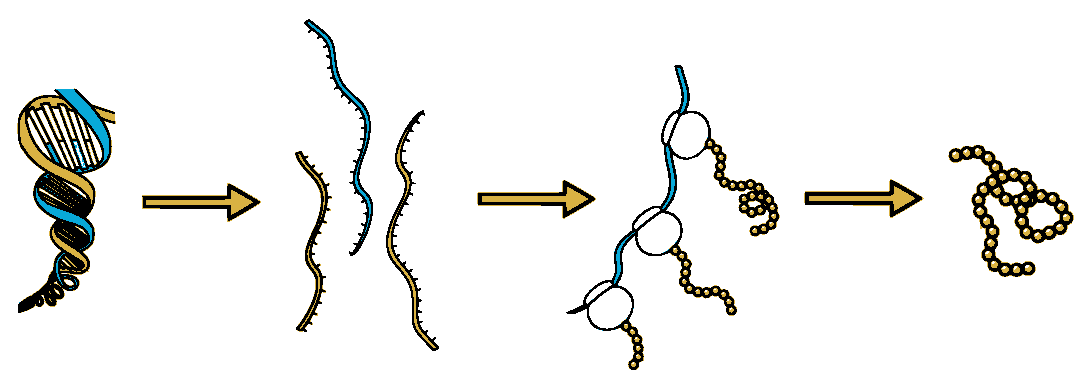
\includegraphics[width=\unitlength]{./img/msms/dna-transcription-translation-divided-text.eps}}%
    \put(0.05002023,0.33543109){\color[rgb]{0,0,0}\makebox(0,0)[lb]{\smash{Transcription}}}%
    \put(0.55348021,0.33543109){\color[rgb]{0,0,0}\makebox(0,0)[lb]{\smash{Traduction}}}%
%    \put(-0.00360921,0.00052073){\color[rgb]{0,0,0}\makebox(0,0)[lb]{\smash{DNA}}}%
%    \put(0.2820496,0.00052073){\color[rgb]{0,0,0}\makebox(0,0)[lb]{\smash{RNA}}}%
%    \put(0.53268515,0.00052073){\color[rgb]{0,0,0}\makebox(0,0)[lb]{\smash{Ribosomes}}}%
%    \put(0.87416237,0.00052073){\color[rgb]{0,0,0}\makebox(0,0)[lb]{\smash{Protein}}}%
    \put(-0.00360921,0.0005){\color[rgb]{0,0,0}\makebox(0,0)[lb]{\smash{DNA}}}%
    \put(0.2820496,0.0005){\color[rgb]{0,0,0}\makebox(0,0)[lb]{\smash{RNA}}}%
    \put(0.53268515,0.0005){\color[rgb]{0,0,0}\makebox(0,0)[lb]{\smash{Ribosomes}}}%
    \put(0.87416237,0.0005){\color[rgb]{0,0,0}\makebox(0,0)[lb]{\smash{Protein}}}%
  \end{picture}%
\endgroup%

%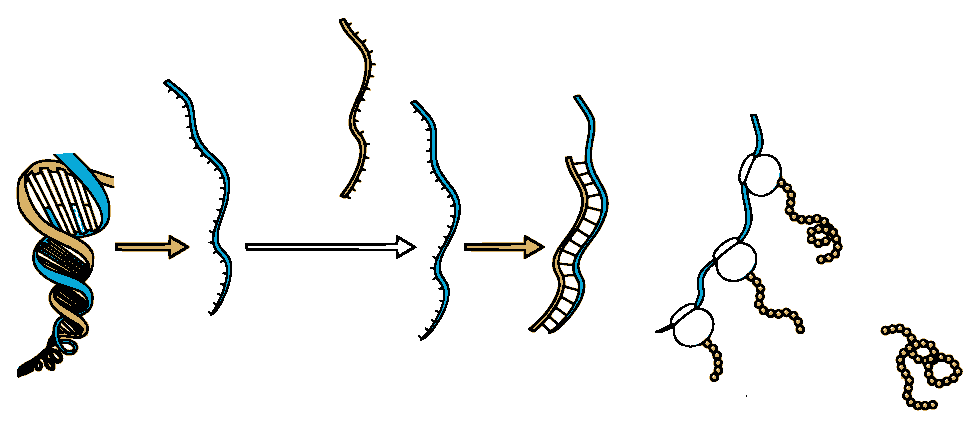
\includegraphics[width=0.7\textwidth]{./img/msms/dna-transcription-translation.eps}
\caption{Schematic representation of the DNA transcription and translation
processes. The information coded in the DNA is transcripted into an messenger
RNA to exit the nucleus where it is stored. Once in the cytoplasm the mRNA is
decoded by ribosomes, the latter assign to each nucleotide triplet a specific
residue, conforming the final polymeric structure of the protein.}
\end{figure}

Proteins fold in stable structures, dominated by
recurring structural motifs, mainly $\alpha$-helices and $\beta$-sheets,
called ``secondary structures''.  
The local regularity of these motifs is related to the strong directionality  of the hydrogen bonds that dictate their geometry.
These motifs are arranged in the global tertiary structure of the folded molecule.
A quaternary structure is defined by proteins complexes where several proteins
are arranged in a functional superstructure.
The above ``structural paradigm'' applies to all proteins with the exception of
the Intrinsically Unfolded Proteins, that are functional in a disordered
conformation; however, such proteins usually get structured upon binding to
their target molecule, so that  we can say that the sequence-structure-function
relationship is still valid, in a loose sense.

\begin{figure}
\begin{center}
\subfigure[primary structure]{
\begin{minipage}{0.3\textwidth}

\includegraphics[width=\textwidth]{./img/2myo-seq.eps}\\
\vskip 5pt
\end{minipage}}
\subfigure[secondary structures]{
\begin{minipage}{0.3\textwidth}
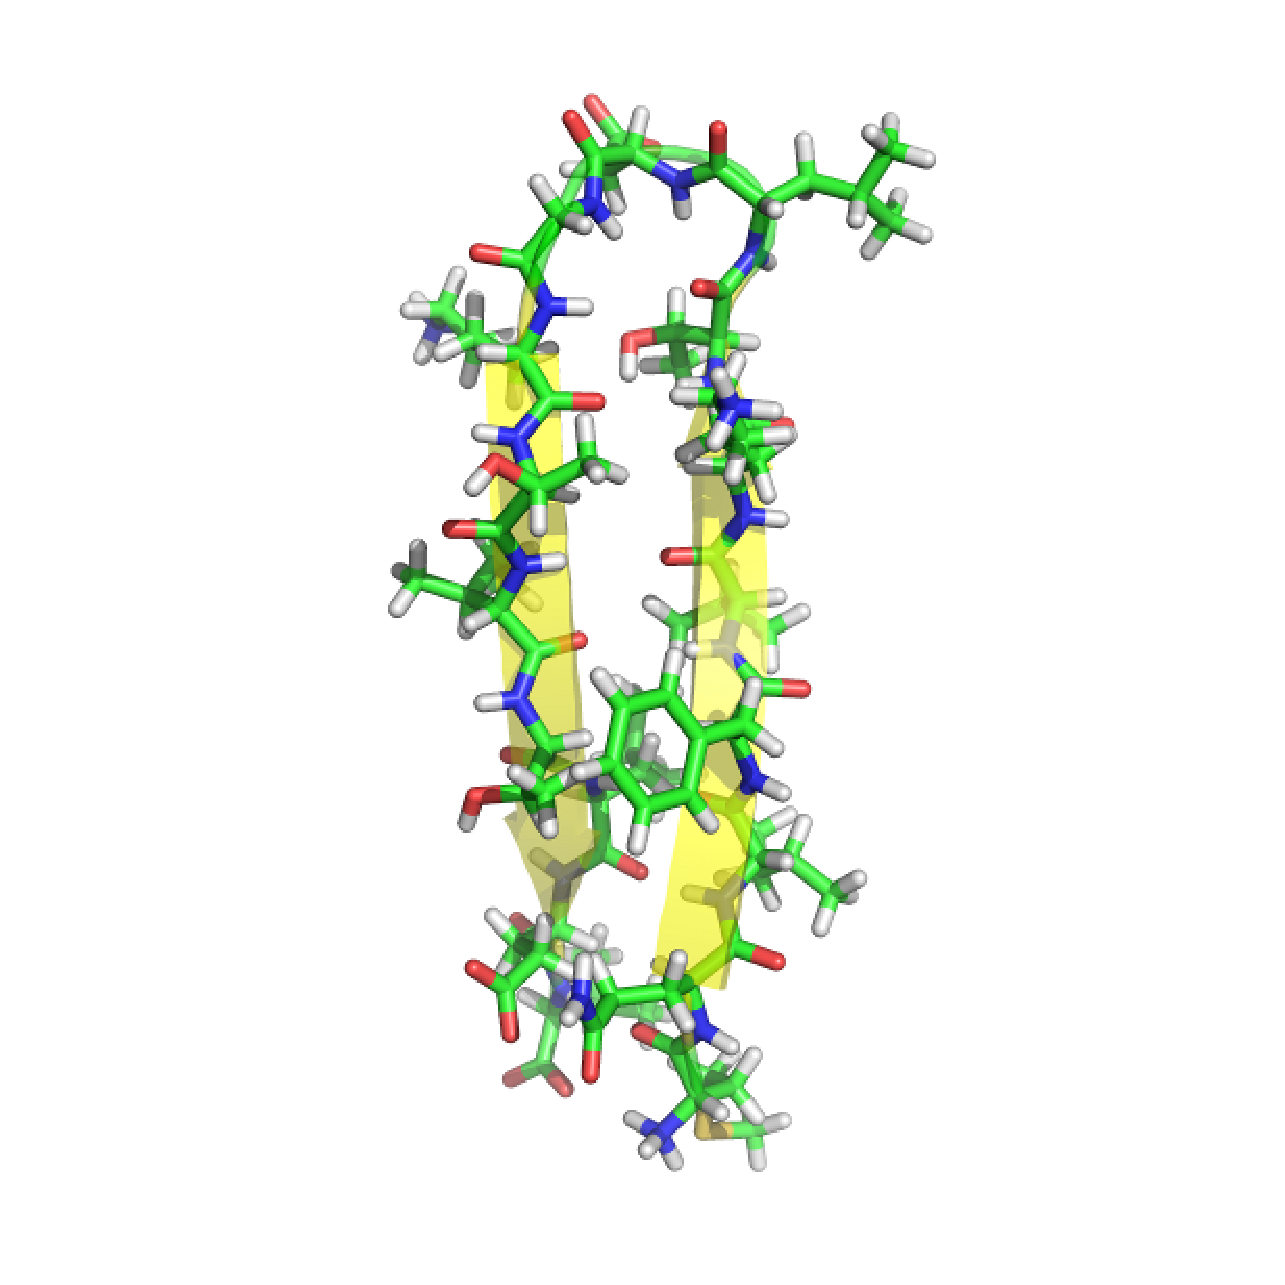
\includegraphics[width=\textwidth]{./img/1e0q-600.eps}\\
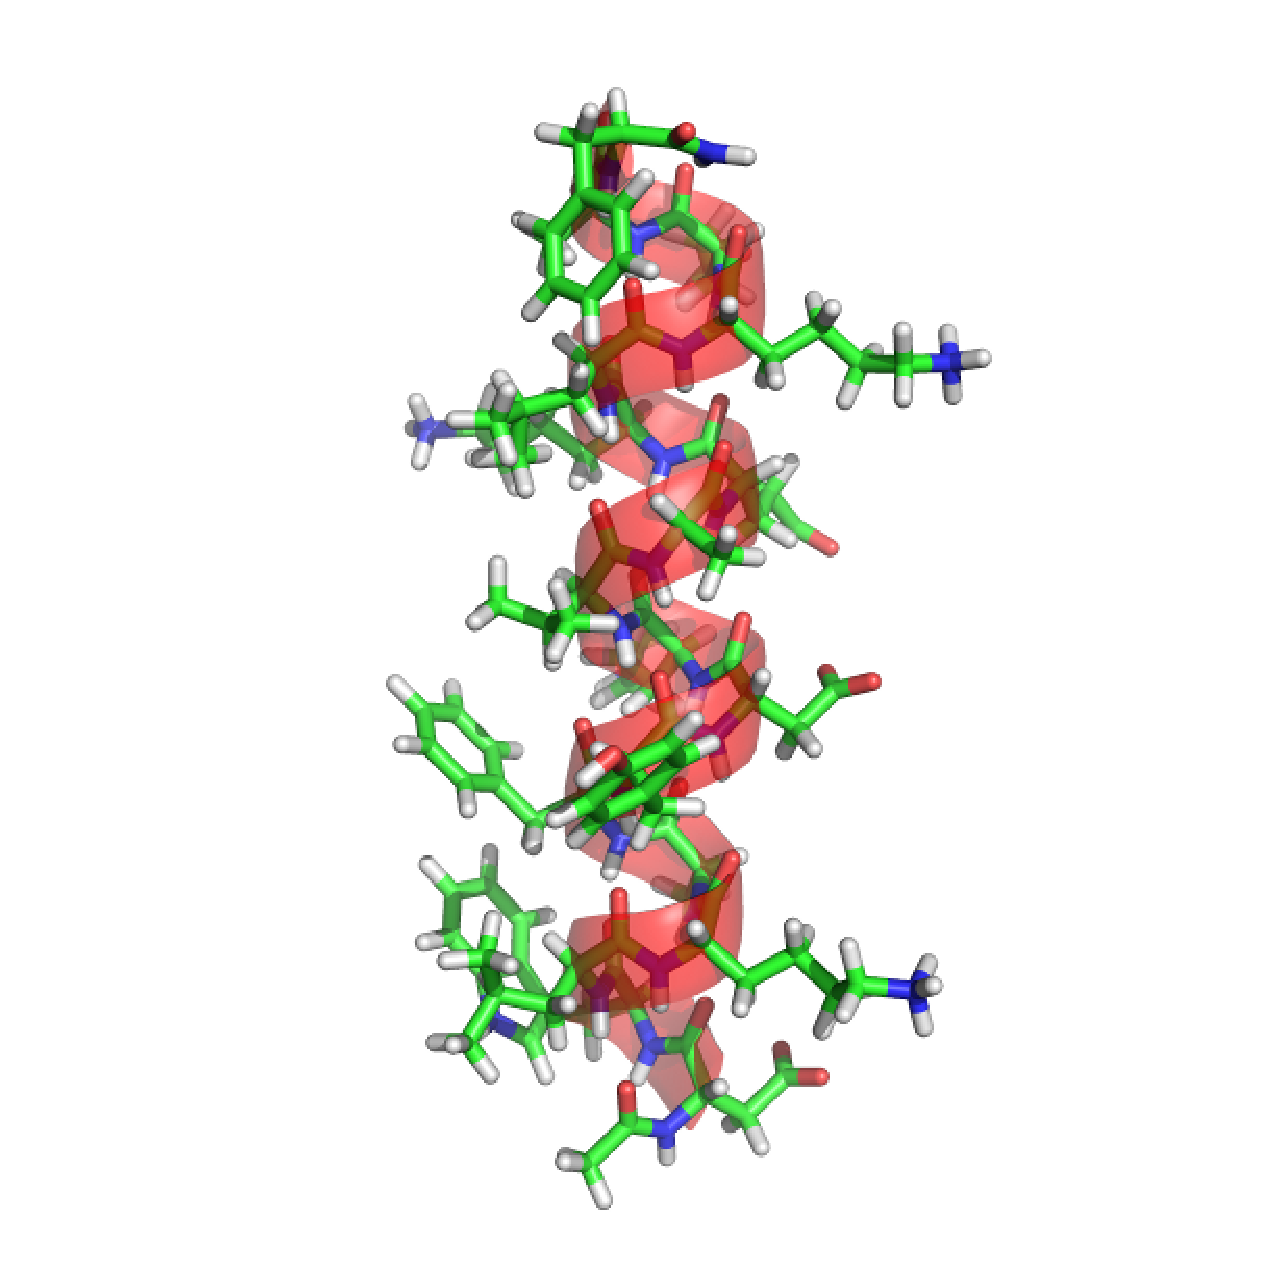
\includegraphics[width=\textwidth]{./img/2fq8-600.eps}
\end{minipage}}
\subfigure[tertiary structure]{
\begin{minipage}{0.3\textwidth}
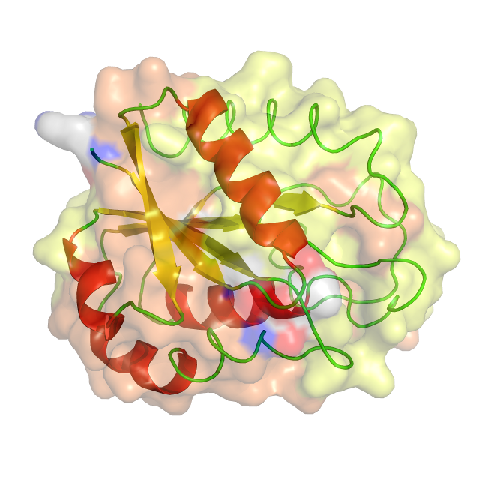
\includegraphics[width=\textwidth]{./img/1flv-600.eps}
\end{minipage}}
\end{center}
\caption{\label{fig:prot-structures}
The polymeric chain of a protein is determined by (a) the residue sequence.
The resulting chain naturally tends to assume a compact structure mainly
conforming (b) structural motifs such as  $\alpha$-helices and
$\beta$-sheets that are arranged on the final (c) native structure.}
\end{figure}

Proteins folds naturally in biological conditions, experiencing an
out-of-equilibrium process that, starting from an unstructured
configuration, ends on the folded native state. 
On the other hand, folding can be studied in vitro under equilibrium and our of
equilibrium conditions: 
from a thermodynamic point of view, the protein native state, in physiological
conditions, represents the stable macro-state, with minimal free-energy; a sudden change to different conditions results in a chemical kinetics that can be usually related to the final free-energy landscape,  and is characterized by the search of the most convenient pathway to reach the new equilibrium. 
In this sense, a folding pathway is specified in terms of the 
% Protein folding is characterized by the pathway followed by the polymer in this process as it describes the 
time dependent formation of the
long-range contacts between non-neighbouring  residues. 

The principal folding  mechanisms that have been identified can be summarized  in
four main behaviours \cite{Nickson2010}: a) Diffusion-Collision: secondary structure folds first and then
the motif diffuse and collide to form the correct structure; b) Hydrophobic Collapse:  
%hydrophobic residues collapse together 
due to the wet environment triggering the folding
process, the protein collapses to a molten globule to protect the non-polar residues from the polar solvent, then the search for the right structure is restricted to compact conformations; c) Nucleation-Propagation: a local nucleus starts the folding process and then propagates to
the entire structure; d) Nucleation-Condensation: the folding nucleus is composed of non-local contacts, involving distant residues along the chain; once a critical number of such contacts is formed, it triggers  the completion of the folding
process. % until it reach a critical number of formed long range contacts.

Different proteins, or even the same protein under different conditions, can show different folding mechanisms.
The detailed characterization of protein folding pathways passes through the
characterization of every conformation that the molecule assumes along the way to the
native state\cite{Daggett2002} and  reflects the picture of the energy landscape. Such characterization  has been successfully achieved  in small proteins combining experimental results with molecular dynamic
simulations: most often, the former 
%However experimental studies of protein folding 
provide snapshots of the
structures along the folding pathway that, although devoid of %they do not provide 
the temporal information on contact formation, can give a picture of the intermediate states
and the overall folding mechanism for the process, while the latter can give insight on the microscopic details of the relevant structures along the folding pathway. 



\paragraph{Protein Sequencing}
In the first part of the Thesis we focus on the problem of peptide
sequencing by Tandem  Mass Spectrometry, which consists in  the interpretation of a mass
spectrum to find the amino-acid sequence  of a target peptide.
Tandem Mass Spectrometry, thanks to its simplicity and low cost, is vastly used in the field of biochemical analysis of unknown
samples of protein, and is 
generally embedded in an automated high-throughput pipeline, which produces a huge
amount of data,  requiring an automated interpretation tool.

In principle,  a Tandem Mass spectrum contains all  the necessary information to find
the peptide sequence it comes from. In practice, reading out the sequence from the spectrum is always a difficult task, complicated by the presence of noise, of peaks from contaminants, and of missing or unexpected fragmentations.  
Actually, each spectrum is the statistical outcome of  the microscopic rules
governing the energy transfer and stochastic fragmentation of the precursor
peptide under collisions, in the presence of contaminants and of noise of
different kind.  Unfortunately, ab-initio predictions of the spectrum given a
precursor ion are  impractical, if not impossible,  and  the identification of
the peptide sequence involves the use of ad-hoc score functions to rate the
agreement between the  theoretical spectrum of a parent peptide and the
experimental one.  Moreover, the search space is usually limited to the
sequences of  known proteins (``database search'' approach), which is more
practical and efficient, but also more limited than de-novo methods which infer
the peptide from just the information contained in the spectrum. 
Finally, it is remarkable that, both for database-search and for de-novo
methods, a central problem is related to assessing the reliability of the
prediction, mainly related to the prediction of  false positives, i.e., wrong
sequences with high scores.

We describe a new algorithm for  protein sequencing based on the mapping of the
interpretation problem onto the analysis of the equilibrium distribution of a
suitably defined discrete physical model, whose dynamic variables describe the
presence of a peptide bond (a fragmentation site) on the sites of a
one-dimensional lattice, labelled by a mass index.
The model is governed by an \emph{ad hoc} energy function,  learned from the
distribution of the ions and of the noise peaks on a dataset of
experimental spectra.  Such Hamiltonian is characterized by just on-site and
nearest-neighbour interactions, so that the partition function of the model can
be exactly calculated by a transfer-matrix approach. While the identification of
the precursor peptide is associated to the characterization of the ground-state
of the model (the zero-temperature solution),
the introduction of a parametric temperature, which represents an original
approach to this problem, and the study of the thermodynamic variables as a
function of the temperature, can give insight on the quality of the
identification, without relying on decoy databases or on phenomenological
distribution of the scores of the false positives.
Indeed, as the temperature increases, the thermodynamic equilibrium shifts from
a regime dominated by the energy and polarized on the best scoring peptide
sequence, to a regime dominated by the entropy coming from  the alternative
sequences with a reasonably good  score on the experimental spectrum.

The resulting algorithm has been applied to a test database of spectra and the results are
reported in this thesis. We show that the performance of this algorithm is
comparable of existing and more popular models, while presents a new valuable
feature: the fictitious temperature that pulls the system outside the energetic
minimum can give the user a tool to estimate the quality of the prediction.


\paragraph{Protein Folding}
In the second part of the Thesis we deal with  the protein folding problem,
focusing in particular on  the characterization of the equilibrium and kinetics
of the repeat protein Myotrophin.
Protein folding is a challenging problem that has been vastly analysed by
theoreticians %physicists and chemists 
using different levels of coarse-graining, % with a wide range of levels of details, 
from all atoms simulations
with realistic interactions, to a variety of coarse grained models.

The protein studied in this work, Myotrophin, is a repeat protein composed by
four modules with the same secondary structure (but different sequence), %composition, 
arranged in a linear way. This kind of structural organization, common to all
repeat proteins,  makes them different from the commonly  studied globular
proteins: in the latter, far apart regions of the sequence can come close (``in
contact'') to one another in the native structure, and the contact range can
span the whole sequence length. On the contrary, in the former, contacts take
place just within a module and between contiguous modules.
Myotrophin
%This conformation experimentally 
shows a challenging behaviour, that has attracted  the attention of the researchers, as the molecule
seems to fold in a cooperative way, which is more typical of a globular protein, while %despite 
its modularity would suggest an intrinsic independence of the conforming
modules, more naturally associated to a multi-state folding, with several
intermediate states corresponding to the folding of independent modules.
Moreover, the experimental results on kinetics have been interpreted in the
framework of the existence of  two alternative folding pathways, labelled
according to which of the two protein ends folds first.

In this work we rely on the Wako- Saito-Mu\~noz-Eaton (WSME) model to characterize the behaviour of
Myotrophin.
This simple model resorts to a binary variable to describe the state (``folded'' or ``unfolded'') of each
residue, and uses the information on the atomic coordinates of the native %the wild type folded 
structure of a protein, stored in a contact map that describes the euclidean proximity of two residues,   to predict its folding behaviour. %describe the global and local behaviour of the polymer through the definition of 
Despite the presence of long-range  interactions  in the energy function of the model, its special form allows the exact evaluation of the partition function, so that equilibrium thermodynamic quantities such as free-energies and heat capacities can be exactly and efficiently calculated, while the dynamics can be studied by Monte Carlo simulations.

We use a slightly modified WSME model to study both the wild type protein and
some mutants; to this purpose, we mimic  single point mutations by changing the
interactions potentials of the mutated residue.
We introduce a new way to characterize, in the folding and unfolding processes,
the relaxation pathways based on the secondary structure formation and denaturation.

 
% of the wild type and qualitatively reproduce the general behaviour of the experimental data.

In both the wild type and mutant proteins, results show a good qualitative agreement with experimental results, with
particular emphasis on the heterogeneity of the folding pathways.
The higher control allowed by  \emph{in silico} simulations over \emph{in vitro}
experiments, and an original way to interpret kinetic data,
 let us shed some light on the subtending processes as the
consistency of the modular structure and free-energy profile and the folding
cooperativity, as well as the lack of  symmetry between the folding and
unfolding pathways.




